\documentclass[a4paper]{scrartcl}
\usepackage[utf8]{inputenc}
\usepackage[english]{babel}
\usepackage{graphicx}
\usepackage{lastpage}
\usepackage{pgf}
\usepackage{wrapfig}
\usepackage{fancyvrb}
\usepackage{fancyhdr}
\pagestyle{fancy}

\usepackage[colorlinks=true,linkcolor=violet]{hyperref}
\usepackage[figure]{hypcap} %jump to img instead of caption text

\def\code#1{\texttt{#1}}


% Create header and footer
\headheight 27pt
\pagestyle{fancyplain}
\lhead{\footnotesize{Network Programming, ID1212}}
\chead{\footnotesize{Homework 4: Currency Converter}}
\rhead{}
\lfoot{}
\cfoot{\thepage\ (\pageref{LastPage})}
\rfoot{}

% Create title page
\title{Homework 4: Currency Converter}
\subtitle{Network Programming, ID1212}
\author{Max Körlinge, korlinge@kth.se}
\date{3 December 2018}

\begin{document}

\maketitle


\section{Introduction}

\noindent This assignment was to develop a three-tier web application using frameworks for all layers. The requested application was a web site where you can convert at least four currencies, optionally together with an admin interface to change current exchange rates. The requirements on the program were:

\begin{itemize}
    \item The program must be designed using a layered architecture and object-oriented design principles.
    \item The converter must be able to convert between at least 4 different currencies.
    \item The client must be a web browser.
    \item All layers in the server must programmed with the help of a framework. The videos connected to the assignment suggest Thymeleaf for the view, Spring for the controller, and Spring/JPA for model and integration layers.
    \item The server must handle transactions.
    \item Conversion rates must be stored in a database.
    \item The user interface must be informative, so the user knows what is going on.
\end{itemize}

The optional task was:

\begin{itemize}
    \item Create an admin interface for the application, where an admin can enter conversion rates between different currencies, and show the total number of currency conversions made by all users together since the application started. Conversion rates and the counter must be stored in the database.
\end{itemize}

The program was written in full by the author of this report, and both the basic and the optional tasks were completed.

\section{Literature Study}

To prepare for this assignment, all video material provided by the course connected to this assignment was viewed together with the code of the sample programs. Important information was gathered on how component-based architecutre, applications servers, and the Spring framework with its IoC container, work.

\section{Method}

\noindent The program was written in Java using the IntelliJ IDE. Maven was used to handle dependencies. MySQL was chosen as the DBMS. Otherwise, the suggested frameworks were used (Thymeleaf, Spring, and JPA).

The timeline was as follows: first, watch the related lectures; second, create a preliminary layered design with skeleton classes, including Spring annotations; third, write the configuration files (\code{application.yml}, \code{pom.xml}, \code{@Config}, etc.) and see that the server program can start without error messages; fourth, create sample HTML documents and a Spring controller to see that Thymeleaf is hooked up and ready to go; fifth, create one logical method call that goes from the view all the way to the bottom of the stack (in this case, the call to show all available currencies); sixth, implement all other functionality required. 

\section{Result}

\noindent The complete source code can be found at \href{https://github.com/fongie/CurrencyConverter}{https://github.com/fongie/CurrencyConverter}.

\begin{itemize}
    \item The program had to be designed using object-oriented design principles. Since Spring tends to steer towards domain-driven design, a version of this was used for the layered architecture, similar to the sample program in the course, with slightly different names. The \code{presentation} layer holds the Spring controllers as well as data holding objects that originate from the view. When it needs logic from the rest of the program, it passes it to a so-called service in the \code{services} layer. This layer can make computations like calculating the conversions, and it also passes on necessery calls to the database. Database logic is handled in the \code{repositories} layer, where Spring repository interfaces are used to handle database calls. Lastly, data from the database is represented in the \code{data} layer, where JPA entities and their read-only DTO versions are located.

        Speaking of read-only DTO versions of entities, they are a way to maintain solid encapsulation in the program, which is also maintained by in general letting all classes keep as small a public interface as possible. High cohesion is maintained by the classes holding to their specific purpose, for example, there are separate controllers and service classes for each page of the application (the admin and the conversion page). This separation also helps to reduce coupling, there is for example no MVC-like controller that often has dependencies all over the place.

    \item The converter had to convert between at least four currencies, and it does. The currencies implemented in the development database are SEK, USD, EUR and GBP, but since all calls to \href{https://github.com/fongie/CurrencyConverter/blob/master/currencyconverter/src/main/resources/templates/convert.html#L40}{list available currencies} and their rates are dynamic and \href{https://github.com/fongie/CurrencyConverter/blob/master/currencyconverter/src/main/java/se/kth/korlinge/currencyconverter/services/ConvertService.java#L70}{loaded} from the database, one could include as many currencies as one would wish by simply adding a few rows to the database. Though, since it was not a requirement to be able to enter new currencies in the admin interface, such database calls to include more currencies would have to be manually made. \href{https://github.com/fongie/CurrencyConverter/blob/master/currencyconverter/src/main/resources/schema.sql}{This} is the development schema.

    \item The client had to be a web browser, and there is not much to be said here - it is. Start the app and browse to \code{localhost:8080} for the converter, or \code{localhost:8080/admin} for the admin interface.

    \item All layers had to be programmed using a framework. The suggested frameworks: Thymeleaf, Spring (Spring Boot with Spring Web and JPA), and JPA were all used.

    \item The server had to handle transactions. Transaction management is \href{https://github.com/fongie/CurrencyConverter/blob/master/currencyconverter/src/main/java/se/kth/korlinge/currencyconverter/config/Config.java#L9}{enabled} to Spring using a \code{Config} class. Then, all classes in the \code{service} layers are \href{https://github.com/fongie/CurrencyConverter/blob/master/currencyconverter/src/main/java/se/kth/korlinge/currencyconverter/services/ConvertService.java#L29}{annotated} with \code{@Transacional}, which means that when a method in such a class is called, a new transaction is automatically started, and it is automatically committed when the method ends. The default setting for exceptions is used, which is that transactions are rolled back if runtimeexceptions occur (we do not throw any exceptions ourselves in these classes).

        The \code{@Transactional} annotation is also used in the \href{https://github.com/fongie/CurrencyConverter/blob/master/currencyconverter/src/main/java/se/kth/korlinge/currencyconverter/repositories/RateRepository.java#L16}{repository} interfaces. These interfaces are always transactional by default, but we add an option which means that the interfaces can only be called when a transaction is already started and running. In practice, that means these interfaces can only be called by the classes in the service layer that start the transactions on method call.

    \item Conversion rates had to be stored in a database. They \href{https://github.com/fongie/CurrencyConverter/blob/master/currencyconverter/src/main/java/se/kth/korlinge/currencyconverter/data/Rate.java}{are}, and as mentioned previously, you can store as many as you wish and they will appear on the website. It is worth mentioning that I envisioned the exchange rates to not necessarily be equal in both directions, meaning, that for example SEK-EUR might not have an inverse rate to EUR-SEK, kind of like on Forex where a currency is worth more when buying than when selling. Thus, there is a rate for both SEK-EUR and for EUR-SEK. \href{https://github.com/fongie/CurrencyConverter/blob/master/currencyconverter/src/main/resources/schema.sql}{Here} is the development schema again.

    \item The user interface had to be informative. Note that it does not say that the user interface has to be pretty, so styling was omitted. There is a sample of the converting and admin interfaces in Figure 1. On the left-most picture, you see the convert page after a successful conversion was made. In the middle, you see that the form is properly validated and an error message is shown if the user enters something invalid. As a side-note, I implemented my first ever custom \href{https://github.com/fongie/CurrencyConverter/blob/master/currencyconverter/src/main/java/se/kth/korlinge/currencyconverter/presentation/conversion/UniqueToAndFrom.java}{annotation} to \href{https://github.com/fongie/CurrencyConverter/blob/master/currencyconverter/src/main/java/se/kth/korlinge/currencyconverter/presentation/conversion/UniqueToAndFromValidator.java}{validate} that you are not trying to convert \href{https://github.com/fongie/CurrencyConverter/blob/master/currencyconverter/src/main/java/se/kth/korlinge/currencyconverter/presentation/conversion/ConversionRequest.java#L10}{to and from} the same currency. On the right-most picture, you see the admin interface after a rate has been changed (it is instantly updated to the new value in the list, previous value was 0.11).

    \item The optional task was to implement the admin interface. It should be apparent from the result of the previous requirements that this was done. Worth mentioning is that I decided to log all acesses in a separate table, where the counter on the admin page is derived from (by counting all rows), to prepare for the case where you could want more statistics from the user history in the future, like, for example, which exchange rate was most popular to exchange to and from.

\end{itemize}

\begin{figure}[h!]
    \begin{center}
        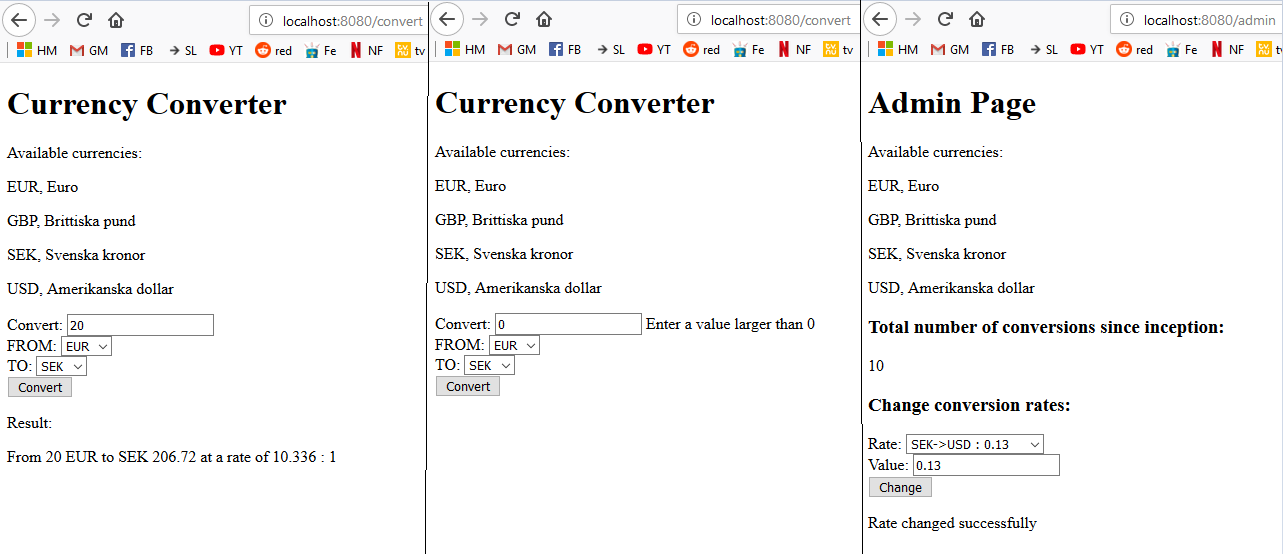
\includegraphics[scale=0.52]{ui.png}
        \caption{A sample output of the user interface}
        \label{fig:ui}
    \end{center}
\end{figure}



\section{Discussion}

This assignment was to develop a three-tier web application using frameworks. It was implemented as a currency converter, where you can convert between currencies, with an admin interface to change exchange rates. Requirements concerned proper object-oriented design and informative user interfaces, as well as using frameworks in all layers to one's advantage. Both the basic and the optional tasks were completed.

Since I have this summer, together with some fellow students, developed a decent size application with a Spring back-end which I coded large parts of, it was not very difficult to get into the Spring related stuff in this assignment. However, that was a REST application (for a React Native mobile interface), so everything regarding Thymeleaf was new and I had to read some documentation to get the templates to where I wanted. I found it quite similar to how XSLT worked in a course last term on XML and databases, so it did not take long to get a grasp of. One part I had not done before was the transaction management, and I hope I got it right. It also inspired me to look at the before-mentioned program we developed in the summer to see if it would benefit from using more than default Spring transaction management. Watching the lectures on how Spring actually works was definately an eye-opener on many things I did not know when using Spring before.

The program could be improved by adding the admin option to add currencies, which would not be difficult and just take a little time, and of course by styling the user interface to be more pleasing to the eye. You could also fetch exchange rates from a public API to get rates that are up-to-date.

\section{Comments About the Course}

I had flow on this assignment and completed it fairly quickly, diving into it straight after finishing the last homework. It took perhaps 2-3 hours on lecture material, 8 hours on code and 2 hours on the report, giving 13 hours in total.

\end{document}
